% lecture01.tex — Smooth Manifolds

\section{Smooth Manifolds}

$\R^k$: $k$-dimensional Euclidean space, i.e.\ a point $x \in \R^k$ is a $k$-tuple $x = (x_1, \ldots, x_k)$ of real numbers.

\begin{definition}{Smooth Map (Open Sets)}{smooth-map-open}
    For open sets $U \subset \R^k$ and $V \subset \R^\ell$, a map $f \colon U \to V$ is called \emph{smooth} (or $C^\infty$) if all the partial derivatives $\frac{\partial^n f}{\partial x_{i_1} \cdots \partial x_{i_n}}$ exist and are continuous.
\end{definition}

More generally, for arbitrary subsets $X \subset \R^k$ and $Y \subset \R^\ell$:

\begin{definition}{Smooth Map (Arbitrary Subsets)}{smooth-map-arbitrary}
    A map $f \colon X \to Y$ is called \emph{smooth} if for each $x \in X$ there exists an open $U \subset \R^k$ containing $x$ and a smooth map $F \colon U \to \R^\ell$ such that $F = f$ on $U \cap X$.
\end{definition}

\begin{center}
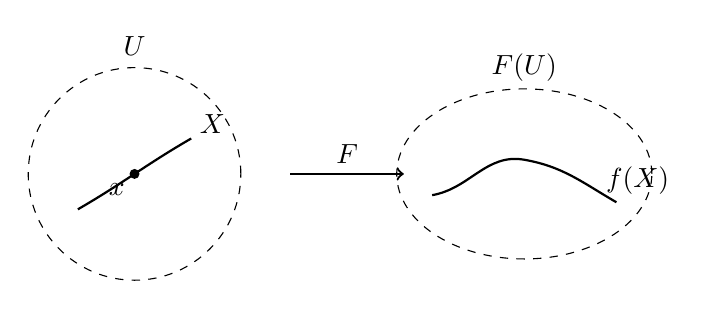
\begin{tikzpicture}[scale=0.9]
    % Left: U containing X with point x
    \draw[dashed] (0,0) circle (1.5);
    \node at (0,1.8) {$U$};
    \draw[thick] (-0.8,-0.5) to[out=30,in=210] (0.8,0.5);
    \node at (1.1,0.7) {$X$};
    \fill (0,0) circle (2pt) node[below left] {$x$};
    % Arrow
    \draw[->,thick] (2.2,0) -- (3.8,0) node[midway,above] {$F$};
    % Right: F(U) containing f(X)
    \draw[dashed] (5.5,0) ellipse (1.8 and 1.2);
    \node at (5.5,1.5) {$F(U)$};
    \draw[thick] (4.2,-0.3) to[out=10,in=170] (5.5,0.2) to[out=-10,in=150] (6.8,-0.4);
    \node at (7.1,-0.1) {$f(X)$};
\end{tikzpicture}
\end{center}

\begin{proposition}{Composition of Smooth Maps}{comp-smooth}
    If $f \colon X \to Y$ and $g \colon Y \to Z$ are smooth, then $g \circ f \colon X \to Z$ is also smooth. \quad (Easy exercise.)
\end{proposition}

\begin{definition}{Diffeomorphism}{diffeomorphism}
    A map $f \colon X \to Y$ is called a \emph{diffeomorphism} if it is bijective and both $f$ and $f^{-1}$ are smooth.
\end{definition}

\begin{remark}{Meta-definition: Differential Topology}{meta-def-diff-top}
    \emph{Differential topology} is the study of properties of ``spaces'' which are invariant under diffeomorphism.
\end{remark}

A particularly nice class of ``spaces'' is:

\begin{definition}{Smooth Manifold}{smooth-manifold}
    A subset $M \subset \R^k$ is called a \emph{smooth manifold of dimension $m$} (or simply a \emph{smooth $m$-manifold}) if it is locally diffeomorphic to $\R^m$, i.e.\ if each $x \in M$ has a neighborhood $W \cap M$ that is diffeomorphic to an open $U \subset \R^m$.

    A diffeomorphism $\phi \colon U \to W \cap M$ is called a \emph{parametrization} of the region $W \cap M$. The inverse diffeomorphism $\phi^{-1} \colon W \cap M \to U$ is called a \emph{coordinate system} on $W \cap M$.
\end{definition}

\begin{example}{The Unit Sphere}{unit-sphere}
    The unit sphere $S^2 = \{(x,y,z) \in \R^3 \mid x^2 + y^2 + z^2 = 1\}$ is a smooth 2-manifold (i.e.\ a smooth surface).

    For instance, the diffeomorphism
    \[
        (x,y) \mapsto (x, y, \sqrt{1 - x^2 - y^2}) \qquad (x^2 + y^2 < 1)
    \]
    parametrizes the region $z > 0$ of $S^2$.

    By interchanging the roles of $x, y, z$ and changing the signs, we obtain parametrizations of regions which cover $S^2$.

    More generally, $S^{n-1} = \{x \in \R^n \mid |x| = 1\}$ is a smooth $(n-1)$-manifold.
\end{example}

\begin{example}{Graph of $y = \sin(1/x)$}{sin-graph}
    $\{(x,y) \in \R^2 \mid x \neq 0,\; y = \sin(1/x)\}$ is a smooth 1-manifold.
\end{example}

\begin{center}
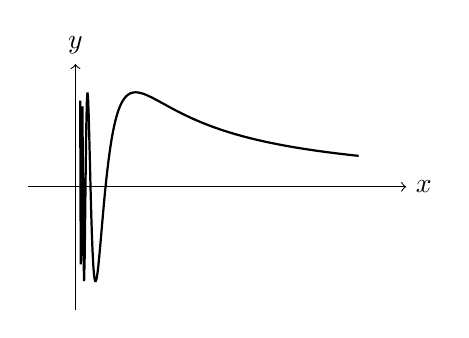
\begin{tikzpicture}[scale=1.2]
    \draw[->] (-0.5,0) -- (3.5,0) node[right] {$x$};
    \draw[->] (0,-1.3) -- (0,1.3) node[above] {$y$};
    \draw[thick,domain=0.05:3,samples=500] plot (\x, {sin(1/\x r)});
\end{tikzpicture}
\end{center}

\begin{remark}{Extrinsic vs.\ Intrinsic Definition}{extrinsic-intrinsic}
    Note that the definition of smooth manifolds we gave is ``extrinsic'' in that $M$ is embedded in $\R^k$. We can also give a better, ``intrinsic'' definition as follows.
\end{remark}

\begin{definition}{Topological Manifold}{topological-manifold}
    A Hausdorff, second countable topological space $M$ is called a \emph{topological $m$-manifold} if it is locally homeomorphic to $\R^m$.
\end{definition}

\begin{definition}{Coordinate Chart}{coordinate-chart}
    A \emph{coordinate chart} is a pair $(U, x)$ consisting of open $U \subset M$ and a homeomorphism $x \colon U \to \R^m$ onto its image.
\end{definition}

Two charts $(U, x)$ and $(V, y)$ on $M$ are \emph{smoothly related} if the transition function $y \circ x^{-1} \colon x(U \cap V) \to y(U \cap V)$ is a diffeomorphism.

An \emph{atlas} on $M$ is a collection $\mathcal{A} = \{(U_\alpha, x_\alpha)\}_{\alpha \in A}$ of smoothly related charts which cover $M$ (i.e.\ $\bigcup_{\alpha \in A} U_\alpha = M$).

A \emph{smooth structure} on $M$ is a maximal atlas. (Any atlas can be completed to a unique smooth structure.)

\begin{definition}{Smooth Manifold (Intrinsic)}{smooth-manifold-intrinsic}
    A \emph{smooth $m$-manifold} is a topological $m$-manifold equipped with a smooth structure.
\end{definition}
